\section{Theoretical Analysis}
\label{sec:analysis}

In this section, the circuit shown in Figure~\ref{fig:rc} is analysed
theoretically, in terms of its time and frequency responses.

\section{Time response}

The circuit consists of a single V-R-C loop where a current $i(t)$ circulates. The
voltage source $v_I(t)$ drives its input, and the output voltage $v_O(t)$ is taken from
the capacitor terminals. Applying the Kirchhoff Voltage Law (KVL), a single
equation for the single loop in the circuit can be written as

\begin{equation}
  Ri(t) + v_O(t) = v_I(t).
  \label{eq:kvl}
\end{equation}

Because $v_O$ is the voltage between capacitor C's plates, it is related to the
current $i$ by
\begin{equation}
  i(t) = C\frac{dv_O}{dt}.
\end{equation}

Hence, Equation~(\ref{eq:kvl}) can be rewritten as
\begin{equation}
  RC\frac{dv_O}{dt} + v_O(t) = v_I.
  \label{eq:kvl2}
\end{equation}

Equation~(\ref{eq:kvl2}) is a linear differencial equation whose solution is a
superposition of a natural solution $v_{On}$ and a forced solution $v_{Of}$:

\begin{equation}
  v_O(t) = v_{On}(t) + v_{Of}(t).
  \label{eq:vo_sol}
\end{equation}

As learned in the theory classes the natural solution is of the form
\begin{equation}
  v_{On}(t) = Ae^{-\frac{t}{RC}},
  \label{eq:vo_nat}
\end{equation}
where $A$ is an integration constant.

The forced solution is of the form given in Equation~(\ref{eq:vo_for}) and is
illustrated in Figure~\ref{fig:forced}.

\begin{equation}
  V_{Of}(t) = |\bar{V}_{Of}| cos(\omega t + \angle \bar{V}_{Of}),
  \label{eq:vo_for}
\end{equation}

\lipsum[1-1]


\begin{figure}[h] \centering
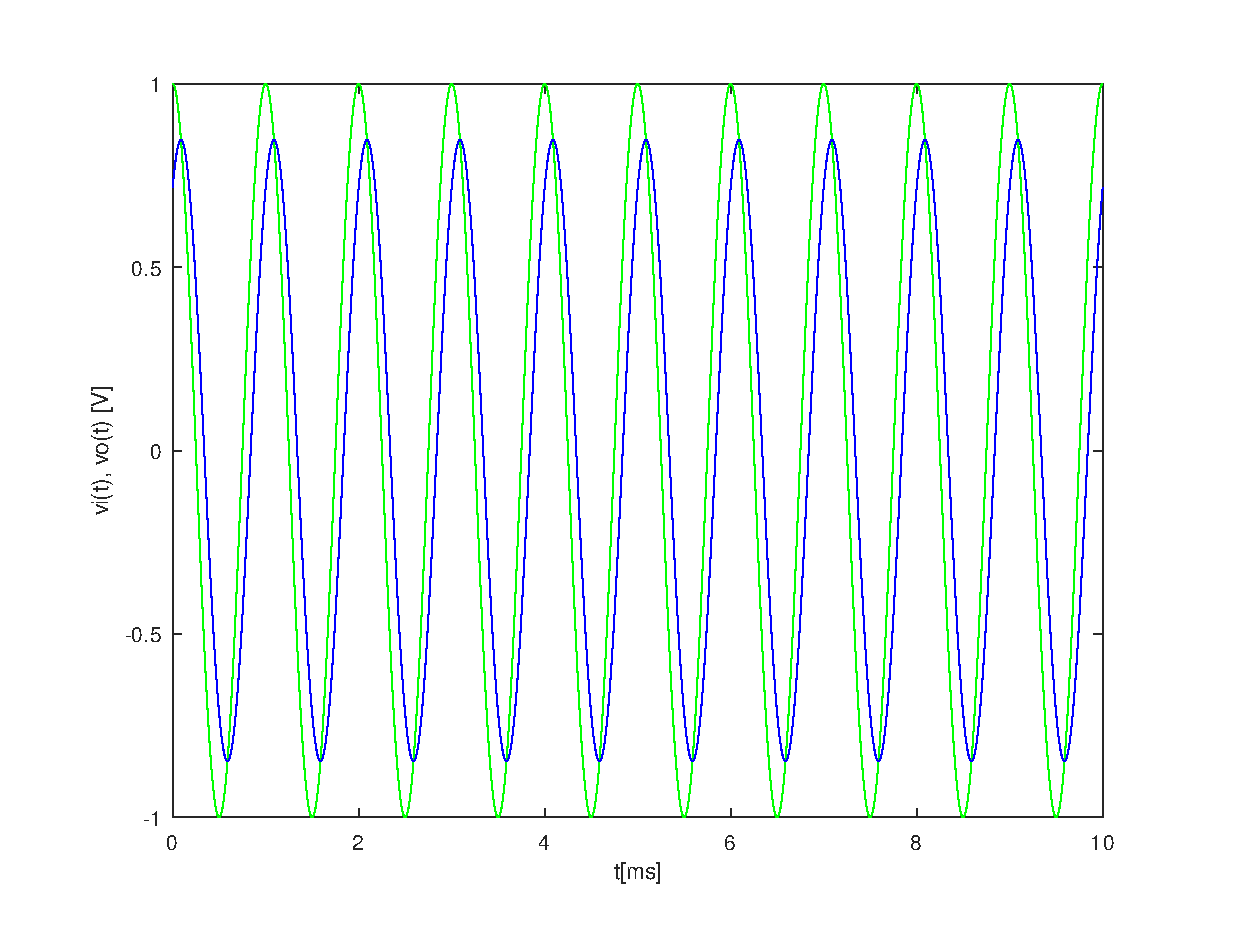
\includegraphics[width=0.8\linewidth]{forced.eps}
\caption{Forced sinusoidal response.}
\label{fig:forced}
\end{figure}

\section{Frequency response}

\lipsum[1-1]


